\section{Simulaci\'on: ecuaci\'on de Schrodinger}
\subsection{Movimiento libre}
Para inicializar la simulaci\'on donde veremos soluciones a la ec. \eqref{eq:schr} entramos en la secci\'on \textit{WavePack Dispersion}.

Para observar un movimiento libre seleccionamos el bot\'on \textit{No} en \textit{Harmonic}, con el slider \textit{Initial position Wavepack} podemos seleccionar la posici\'on inicial de nuestro paquete de ondas. En \textit{excitation of the state} seleccionamos uno de los autoestados dados por la ec. \eqref{eq:sol_schr} y \textit{Number of oscilations} nos permite controlar el tiempo de la simulaci\'on, este tiempo est\'a escalado con el periodo del paquete de ondas bajo un potencial de $w=1$, ahora seleccionamos el bot\'on \textit{START}. Una vez terminada la computaci\'on, principalmente nos interesar\'a la ventana \textit{DISPERSION}. En ella se muestra el c\'alculo de la dispersi\'on para la funci\'on de onda en el espacio R y K, vemos como incrementa con el tiempo para R y constante para K. Seguidamente podemos ver la evoluci\'on de nuestro estado. Utilizando el slider debajo de la gr\'afica o los botones \textit{GO ON, GO BACK, PAUSE} podemos controlar la evoluci\'on del estado. Vemos como ciertamente nuestra funci\'on de onda en el espacio K no sufre ning\'un tipo de dispersi\'on pero en el espacio R s\'i.

\subsection{Oscilador arm\'onico}

Para activar el movimiento oscilatorio arm\'onico solamente debemos presionar el bot\'on \textit{YES} en \textit{HARMONIC}. En esta secci\'on nos centraremos en dos puntos:
\\

(I) Comprobar que el paquete de ondas sigue un movimiento oscilatorio arm\'onico.

(II) Comprobar la cuantizaci\'on de la energ\'ia dada por la ec.  ~\eqref{eq:energ}.
\\

Para obtener los resultados del apartado (I) posicionaremos el paquete de ondas en una posici\'on diferente de 0, se puede elegir el nivel de excitaci\'on que uno desee y ejecutaremos el programa para un tiempo dado. Una vez haya terminado la computaci\'on podemos seleccionar la gr\'afica\textit{ ENERGY}. En ella podemos ver tres valor de la energ\'ia: cin\'etica, potencial y total. Podemos observar una oscilaci\'on como la que cumplir\'ia una part\'icula bajo un potencial arm\'onico, como la de la Fig.~\ref{Fig:harm} . Ahora entramos en la evoluci\'on del estado, ya se ha comentado anteriormente como entrar. En \'el, podemos ver completamente un movimiento oscilatorio. Vemos que, cuando la funci\'on de onda en el espacio R est\'a en un extremo, en el espacio K est\'a en 0 y a la inversa, muestra de un movimiento oscilatorio. En este punto uno ser\'ia capaz de extraer el per\'iodo del movimiento entrando en \textit{MEAN VALUE} donde est\'a calculado el valor medio de la posici\'on del paquete siguiendo la ec ~\eqref{eq:mean} y as\'i compararlo con el resultado te\'orico.
\linebreak

\begin{figure}[tb]
	\centering
	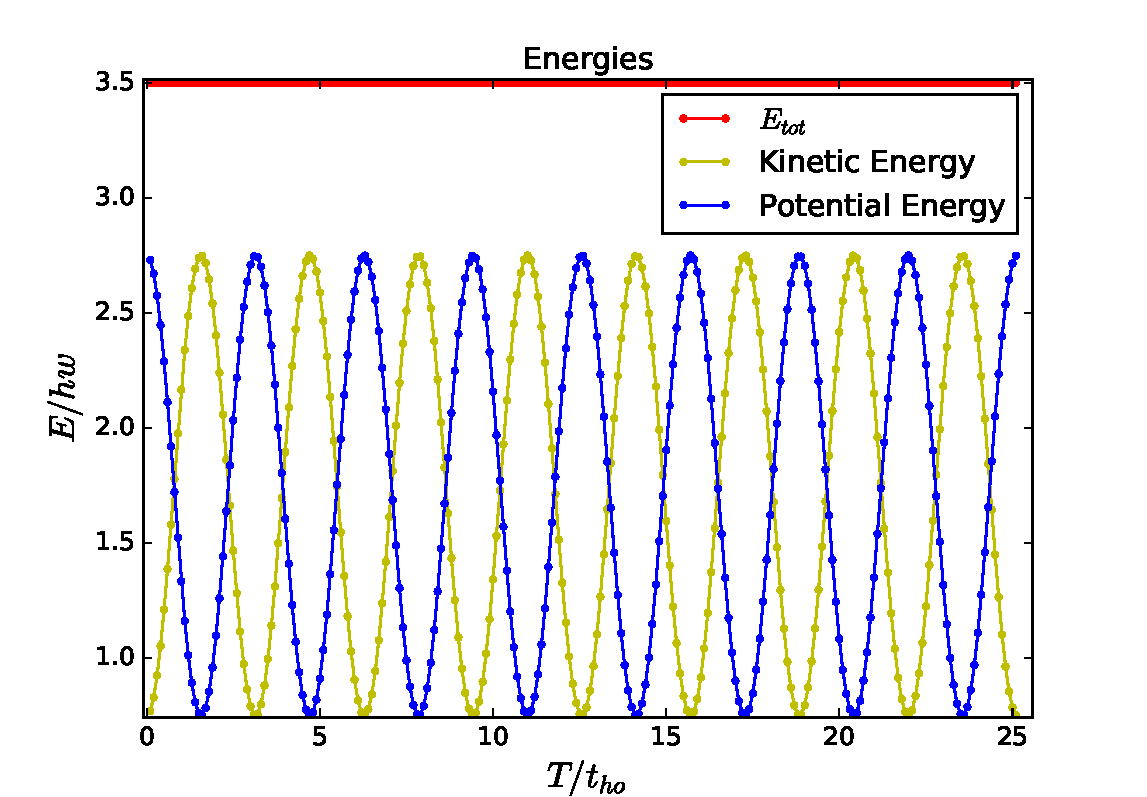
\includegraphics[width=0.9\linewidth]{harm.pdf}
	\caption{Energ\'ias para una funci\'on de onda sometida a un potencial arm\'onico}
	\label{Fig:harm}
\end{figure}
Ahora analicemos el punto (II). La configuraci\'on inicial adecuada ser\'ia: poner el paquete de ondas en la posici\'on 0, introducir un tiempo que queramos y, lo m\'as importante seleccionar el nivel de excitaci\'on, empezaremos con el nivel 0. Una vez finalizados los c\'alculos entramos en \textit{ENERGY}, esta vez, nos interesa la energ\'ia total. Ahora podemos comparar este valor con el dado por la ec. ~\eqref{eq:energ} para $n=0$, ahora reiteramos para $n=1,2$. Tambi\'en podemos comprobar viendo la evoluci\'on del estado que es un propio y por lo tanto, estacionario.
